% Matteo Kumar, Leonard Schatt
% Physikalisches Praktikum


\chapter{Methods, setup and materials}
\label{chap:methods}

In this chapter the used setup, methods and materials are introduced.

\section[Absorption measurement]{Setup for X-ray absorption measurement}

To measure the emission spectrum of the anode, a setup as shown in \cref{fig:setupabs} is used. The X-rays are generated in an X-ray tube (RR). A monochromator, realized in a rotatable single crystal (K), 
selects a specific wavelength of the X-ray spectrum depending on the angle 2$\theta$ set. After an aperture (B), the now nearly monochromatic X-ray radiation hits the sample holder (F). Into this holder the sample
can be inserted. After the radiation passed the sample holder, the intensity of the radiation is measured by a counting tube (Z) and the data is transferred to a computer.

\begin{figure}[h]
    \centering
    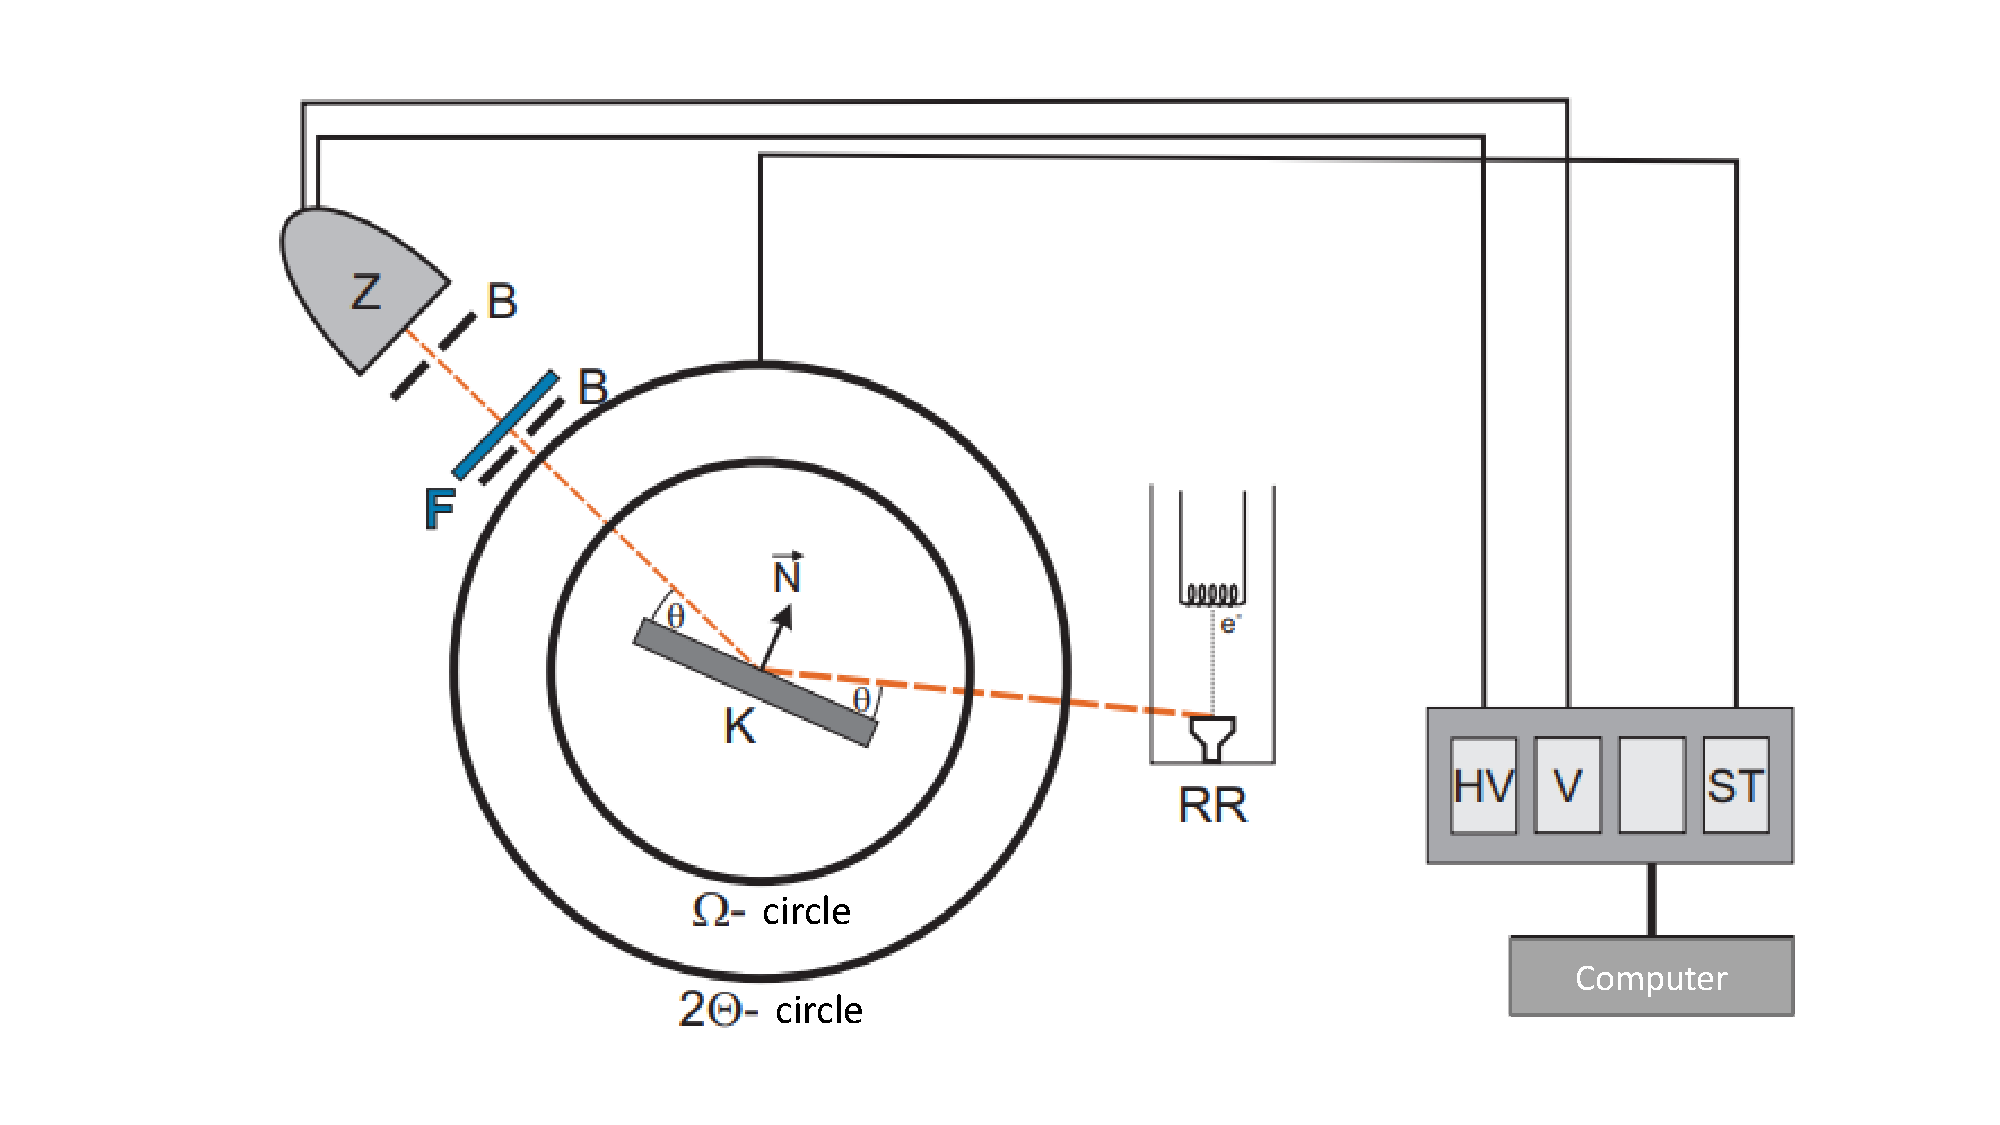
\includegraphics[width =\textwidth]{Bilder/Setup/SetupAbsorb.pdf}
    \caption{Experimental setup of the absorption measurement}
    \label{fig:setupabs}
\end{figure}


\section[Diffraction measurement]{Setup for X-ray absorption measurement}

For the diffraction measurement we are using a similar setup to the setup used before. As depicted in \cref{fig:setupdiff}, the X-rays are generated in an X-ray tube (RR). Afterwards a monochromator selects one X-ray wavelength. 
The sample (S) is turned as the single crystal in the absorption setup. For each position the diffraction under 2$\theta$ is measured measured by a counting tube (Z) and the data is transferred to a computer.

\begin{figure}[h]
    \centering
    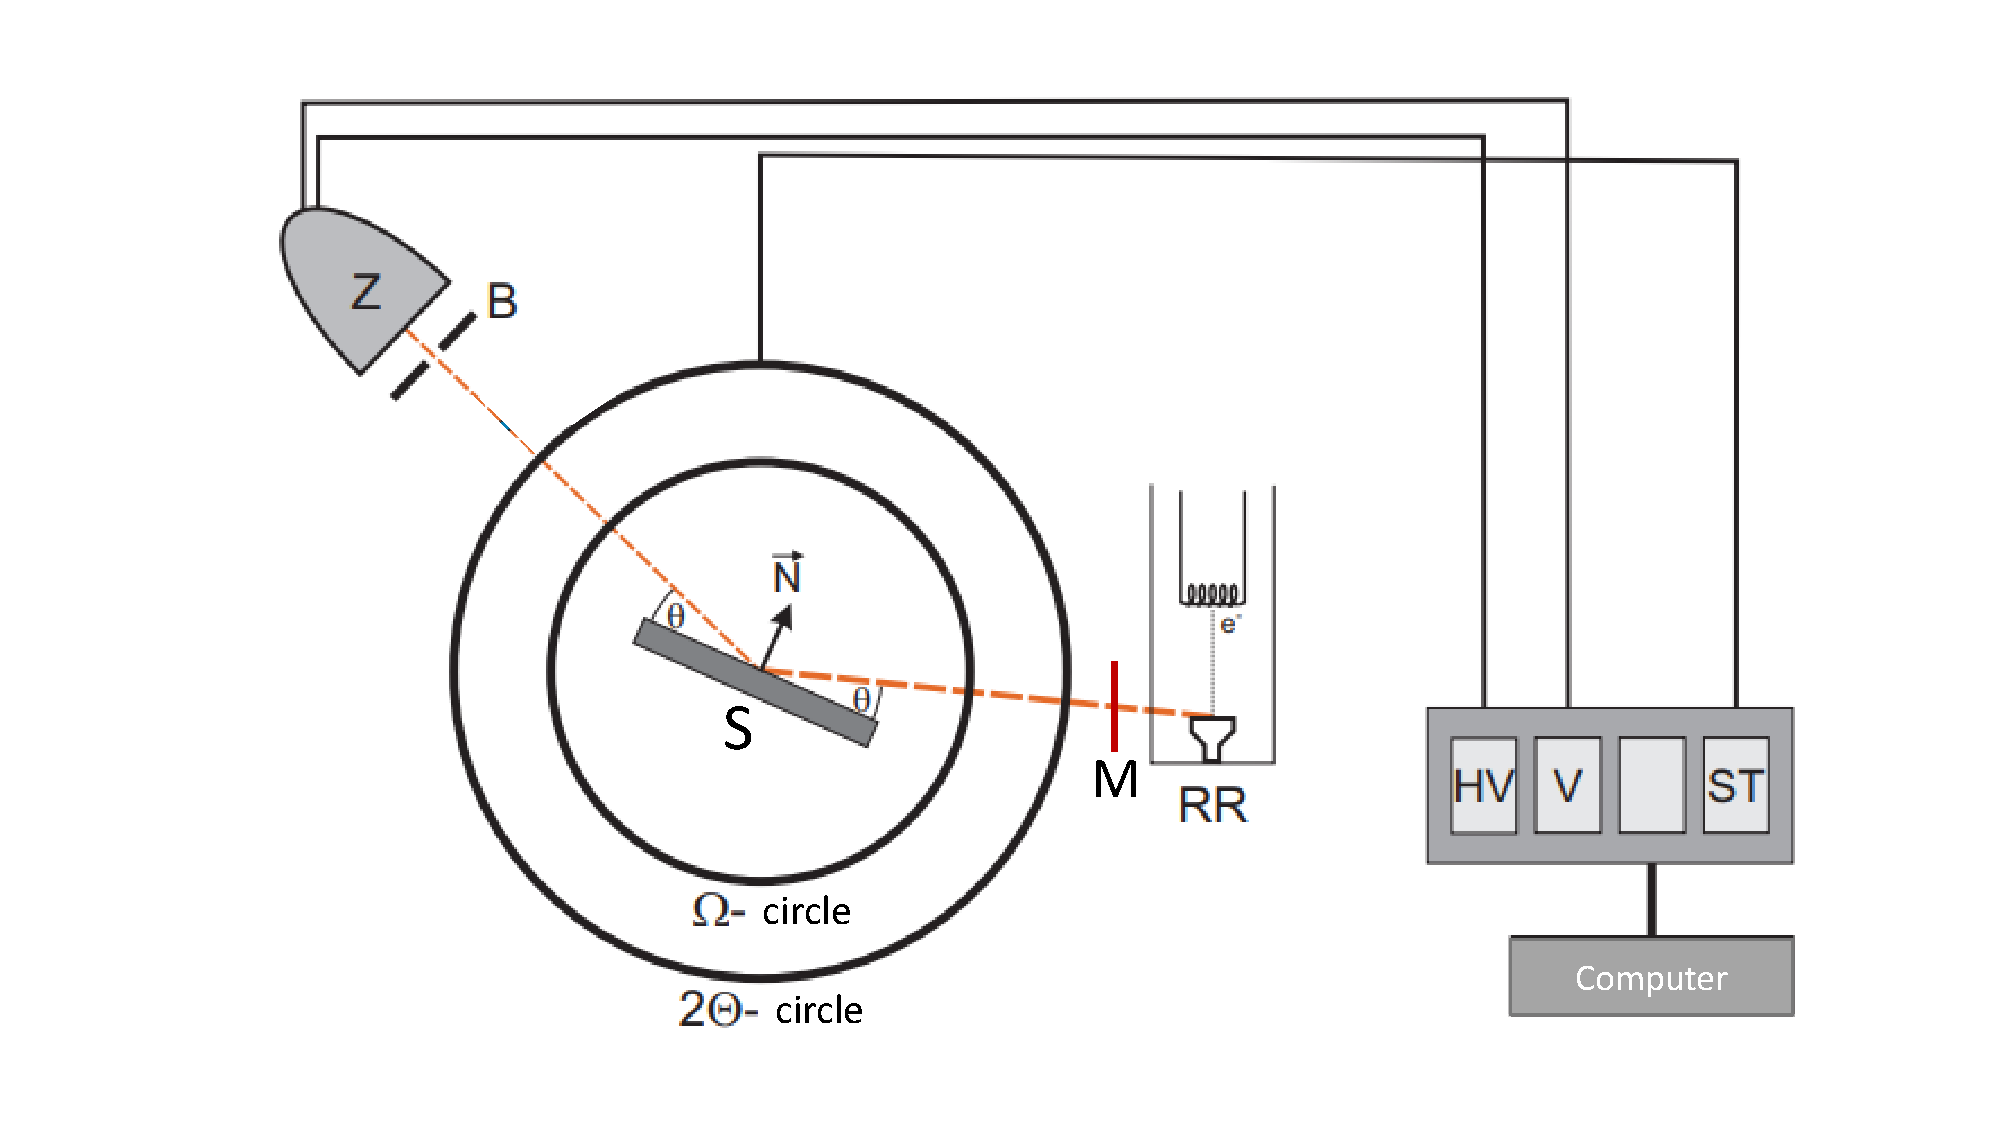
\includegraphics[width = \textwidth]{Bilder/Setup/SetupDiff.pdf}
    \caption{Experimental setup of the diffraction measurement}
    \label{fig:setupdiff}
\end{figure}

In the sample preparation procedure, the crystal under examination (e.g., NaCl, glucose) is finely ground using a mortar. The resulting powder should possess a fine texture, barely detectable when rubbed between the fingers. Subsequently, the powder is carefully loaded into a sample holder, paying attention to a flat surface of the powder. Finally, the sample holder is inserted into the X-ray setup and the measurement is started. The measurement process runs for
approximately one week.